\documentclass[12pt]{beamer}

\mode<presentation>{\usetheme{Warsaw}}
\setbeamertemplate{footline}[frame number]
\usepackage[english]{babel}
\usepackage{times}
\usepackage{url}
\usepackage{graphicx}
\usepackage{listings}
\lstloadlanguages{Python}
\lstset{language=Python}
\lstset{%
	basicstyle=\ttfamily\bfseries,
	keywordstyle=\color{blue}, emph={self}, emphstyle={\color{blue}},
	identifierstyle=,
	commentstyle=\color{gray},
	stringstyle=\color{green!50!black},
	showstringspaces=false,
	emph={[2]__init__,__str__}, emphstyle={[2]\color{purple}},
}
\newcommand{\key}[1]{{\color{blue}#1}}
\newcommand{\cmnt}[1]{{\color{gray}#1}}
\newcommand{\str}[1]{{\color{green!50!black}#1}}
\newcommand{\defn}[1]{{\color{purple}#1}}
\newcommand{\V}[1]{\mbox{\texttt{#1}}}

\title{Constraint Satisfaction Problems}
\subtitle{Introduction to Artificial Intelligence}
\author{Steven Bethard}
\institute{
  Department of Computer Science\\
  University of Colorado
}
\date{CSCI 3202}

\AtBeginSection[]{
  \begin{frame}<beamer>{Outline}
    \tableofcontents[currentsection]
  \end{frame}
}

\begin{document}

\begin{frame}
  \titlepage
\end{frame}

\begin{frame}{Outline}
  \tableofcontents
\end{frame}

\section{Constraint Satistfaction}

\subsection{Example Problem}
\begin{frame}{Meeting Scheduling}
	\begin{block}{Daily Meetings}
		\begin{itemize}
			\item Jim \& Tammy for 2 hours
			\item Jim \& Martha for 1 hour
			\item Martha \& Tammy for 1 hour
		\end{itemize}
	\end{block}
	\begin{block}{Constraints}
		\begin{itemize}
			\item Between 9:00am and 5:00pm
			\item Each person needs 1 hour between meetings
			\item Busy: Jim 12-2, Martha 11-1, Tammy 10-11 and 2-3
		\end{itemize}
	\end{block}
\end{frame}

\subsection{Formal Definition}
\begin{frame}{Constraint Satisfaction Problem Definition}
	\begin{block}{Terms}
		\begin{description}
			\item[Variables] $X_1, X_2, \ldots, X_n$
			\item[Domains] Allowable values for each variable
			\item[Constraints] Allowable combinations of variables
		\end{description}
	\end{block}
	\begin{block}{States}
		\begin{description}
			\item[Assignment] of values to variables, $\{X_i=v_i, X_j=v_j, \ldots\}$
		\end{description}
	\end{block}
	\begin{block}{Types of States}
		\begin{description}
			\item[Consistent] No constraints violated
			\item[Solution] No constraints violated, all variables assigned
		\end{description}
	\end{block}
\end{frame}
\begin{frame}{Map Coloring}
	\begin{columns}
		\begin{column}{1.5in}
			\begin{block}{Problem}
				Color all countries with red, green or blue,
				and with no 2 adjacent countries the same color
			\end{block}
		\end{column}
		\begin{column}{2.5in}
			\only<1>{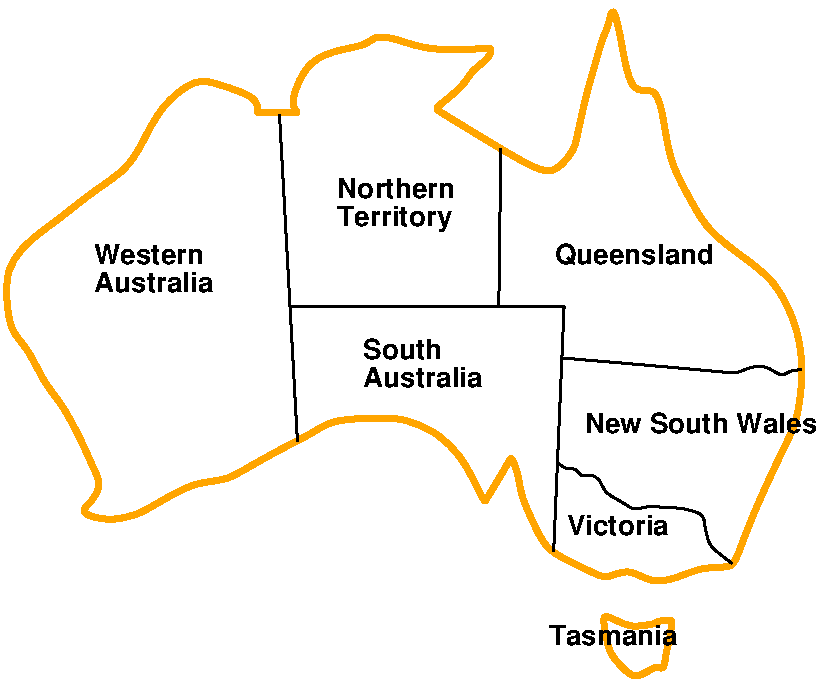
\includegraphics[height=1.75in]{australia.pdf}}%
			\only<2->{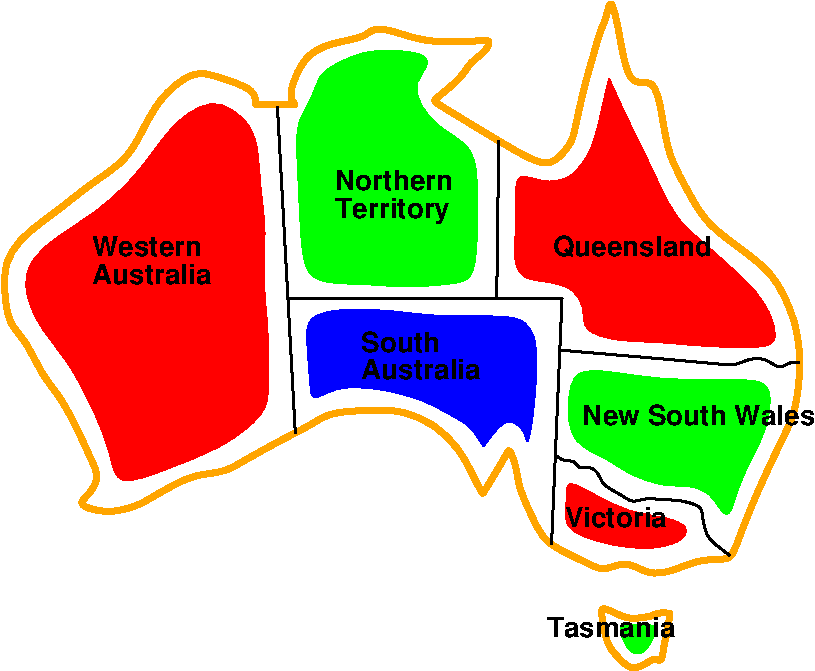
\includegraphics[height=1.75in]{australia-solution.pdf}}%
		\end{column}
	\end{columns}
	\begin{description}
		\item[Variables] \uncover<3->{\V{WA}, \V{NT}, \V{Q}, \V{NSW}, \V{V}, \V{SA}, \V{T}}
		\item[Domains] \uncover<4->{$D_i = \{\V{red}, \V{green}, \V{blue}\}$}
		\item[Constraints] \uncover<5->{$\V{WA} \neq \V{NT}, \V{WA} \neq \V{SA}, \V{NT} \neq \V{SA}, \ldots$}
		\item[Solution] \uncover<6->{$\{\V{WA}=\V{red}, \V{NT}=\V{green}, \V{Q}=\V{red}, \linebreak
		                                \V{NSW}=\V{green}, \V{V}=\V{red}, \V{SA}=\V{blue}, \linebreak
		                                \V{T}=\V{green}\}$}
	\end{description}
\end{frame}
\begin{frame}{Visualizing Constraints}
	\begin{block}{Constraint Graph}
		\begin{itemize}
			\item Nodes are variables
			\item Edges are constraints between variables
		\end{itemize}
	\end{block}
	\hspace{0.5in}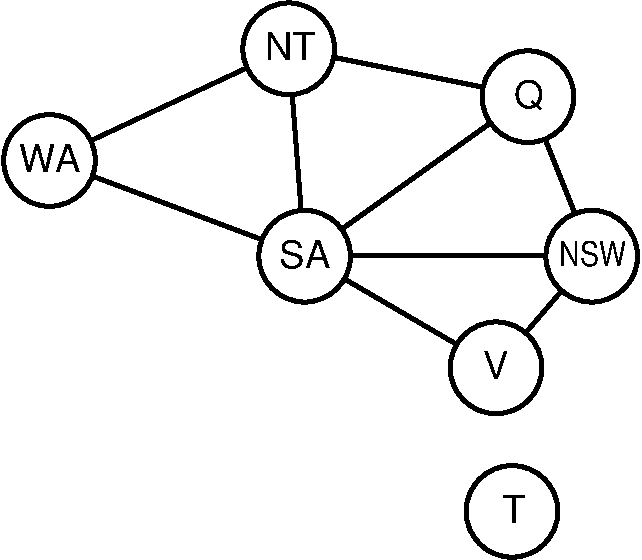
\includegraphics[height=2in]{australia-csp.pdf}
\end{frame}
\begin{frame}{Meeting Scheduling}
	\begin{block}{Problem Description}
		\begin{itemize}
			\item 2 hour meetings: Jim \& Tammy
			\item 1 hour meetings: Jim \& Martha, Martha \& Tammy
			\item 9:00am and 5:00pm, 1 hour between meetings
			\item Busy: Jim 12-2, Martha 11-1, Tammy 10-11 and 2-3
		\end{itemize}
	\end{block}
	\begin{description}
		\item[Variables] \uncover<2->{\V{J\&T}, \V{J\&M}, \V{M\&T}}
		\item[Domains] \uncover<3->{
			$D_{\V{\scriptsize J\&T}} = \{\V{9-11}, \V{10-12}, \ldots\}$ \\
			$D_{\V{\scriptsize J\&M}} = D_{\V{\scriptsize M\&T}} = \{\V{9-10}, \V{10-11}, \ldots\}$}
		\item[Constraints] \uncover<4->{
			$\V{J\&T} \cap \V{J\&M} = \V{J\&M} \cap \V{M\&T} = \ldots = \emptyset$ \\
			$\V{12-2} \cap \V{J\&T} = \V{12-2} \cap \V{J\&M} = \ldots = \emptyset$ \\
			\ldots}
		\item[Solution] \uncover<5->{
			$\{\V{J\&T}=\V{3-5}, \V{M\&T}=\V{1-2}, \V{J\&M}=\V{10-11}\}$}
	\end{description}
\end{frame}

\subsection{Problem Types}
\begin{frame}{Domain Types}
	\begin{block}{Finite Domains}
		\begin{itemize}
			\item Examples: map coloring, 8-queens
			\item Constraints described by enumeration, e.g. \\
			      $(\V{WA}, \V{NT}) \in \{(\V{red}, \V{green}), (\V{red}, \V{blue}), \ldots\}$
		\end{itemize}
	\end{block}
	\pause
	\begin{block}{Infinite but Countable Domains}
		\begin{itemize}
			\item Examples: scheduling jobs by day or hour
			\item Need a constraint language, e.g. \\
			      $\V{Start}_{\V{\scriptsize Job1}} + 5 \leq \V{Start}_{\V{\scriptsize Job3}}$
		\end{itemize}
	\end{block}
	\pause
	\begin{block}{Continuous Domains}
		\begin{itemize}
			\item Examples: scheduling jobs by any fraction of time
			\item Some can be solved by linear programming
		\end{itemize}
	\end{block}
\end{frame}
\begin{frame}{Constraint Types}
	\begin{block}{Unary Constraints}
		\begin{itemize}
			\item Restrict the value of a single variable
			\item<2-> Can be eliminated by preprocessing domains
		\end{itemize}
	\end{block}
	\begin{block}<3->{Binary Constraints}
		\begin{itemize}
			\item Relate two variables, e.g. $\V{SA} \neq \V{NSW}$
		\end{itemize}
	\end{block}
	\pause
	\begin{block}<4->{Higher Order Constraints}
		\begin{itemize}
			\item Relate more than two variables
			\item<5-> Can always be broken down into binary constraints
		\end{itemize}
	\end{block}
	\begin{block}<6->{Preferences}
		\begin{itemize}
			\item Cost of assignments, e.g. \V{red} is better than \V{green}
		\end{itemize}
	\end{block}
\end{frame}
\begin{frame}{Cryptarithmetic}
	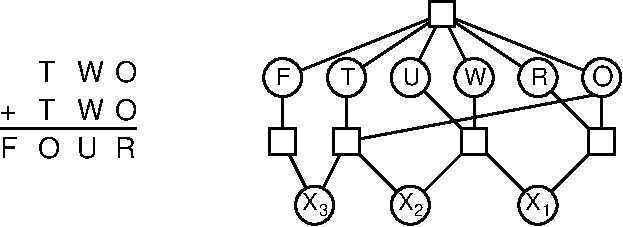
\includegraphics[width=4in]{cryptarithmetic.pdf}
	\begin{description}
		\item[Variables] \uncover<2->{$T, W, O, F, U, R, X_1, X_2, X_3$}
		\item[Domains] \uncover<3->{$\{0, 1, 2, 3, 4, 5, 6, 7, 8, 9\}$}
		\item[Constraints] \uncover<4->{$
			\begin{array}[t]{lll}
			O + O       & = & R + 10 \cdot X_1 \\
			X_1 + W + W & = & U + 10 \cdot X_2 \\
			X_2 + T + T & = & O + 10 \cdot X_3 \\
			X_3         & = & F
			\end{array}
			$}
		\item[Solution] \uncover<5->{$\{T=7, W=3, O=4, F=1, U=6, R=8\}$}
	\end{description}
\end{frame}

\section{Backtracking Search}

\subsection{CSPs as Search}
\begin{frame}{CSPs as Search}
	\begin{block}{Formulation}
		\begin{description}
			\item[States] Full or partial assignments
			\item[Initial] The empty assignment, $\{\}$
			\item[Actions] Assign value to variable, obeying constraints
			\item[Goal] Assignment is complete
		\end{description}
	\end{block}
	\begin{block}<2->{Benefits}
		\begin{itemize}
			\item Same for all CSPs
			\item All solutions at depth $n$ \\
			      \uncover<3->{$\Rightarrow$ depth-first search ok}
		\end{itemize}
	\end{block}
\end{frame}
\begin{frame}{CSPs as Search}
	\begin{block}{Problem}
		Given $n$ variables, $d$ values in domains:
		\\ \smallskip
		\begin{tabular}{|lllll|}
			\hline
			                     & \color{blue}Root & \color{blue}Level 1 & \color{blue} Level 2 & \color{blue}\ldots \\
			\color{blue}Branches & \pause $nd$      & \pause $(n - 1)d$   & \pause $(n - 2)d$    & \ldots \\
			\hline
		\end{tabular}
		\\ \smallskip
		\pause Leaves: \pause $n! \cdot d^n$ \pause \hspace{2em} Total possible assignments: \pause \alert{$d^n$}
	\end{block}
	\pause
	\begin{block}{Note}
		Variable assignments are commutative, e.g.
		\begin{itemize}
			\item $\V{WA}=\V{red}$ then $\V{NT}=\V{green}$
			\item $\V{NT}=\V{green}$ then $\V{WA}=\V{red}$
		\end{itemize}
	\end{block}
	\pause
	\begin{block}{Solution}
		Consider only one variable at each node
	\end{block}
\end{frame}
\begin{frame}[fragile]{Backtracking Search Code}
	\scriptsize
	\begin{semiverbatim}\bfseries
		\key{def} \defn{csp_search}(csp, heuristic, assignment=\key{None}):
		    \pause\key{if} assignment \key{is} \key{None}:
		        assignment = \{\}
		    \pause\cmnt{# if assignment is complete, return it}
		    \key{if} len(assignment) == len(csp.variables):
		        \key{return} assignment
		    \pause\cmnt{# select an unassigned variable and order the values}
		    variable = heuristic.select_variable(csp, assignment)
		    values = heuristic.order_values(csp, assignment, var)
		    \pause\cmnt{# try assigning each value to the variable}
		    \key{for} value \key{in} values:
		        assignment[variable] = value
		        \pause\cmnt{# for consistent assignments, recursively check if
		        # it is possible to assign the remaining variables}
		        \key{if} csp.is_consistent(assignment):
		            result = csp_search(csp, heuristic, assignment)
		            \key{if} result \key{is} \key{not} \key{None}:
		                \key{return} result
		        \pause\key{del} assignment[variable]
		    \cmnt{# all assignments failed}
		    \key{return} \key{None}
	\end{semiverbatim}
\end{frame}
\begin{frame}{Backtracking Example}
	\begin{center}
		\only<1>{
\includegraphics[width=4in]{backtrack-progress-1}}%
		\only<2>{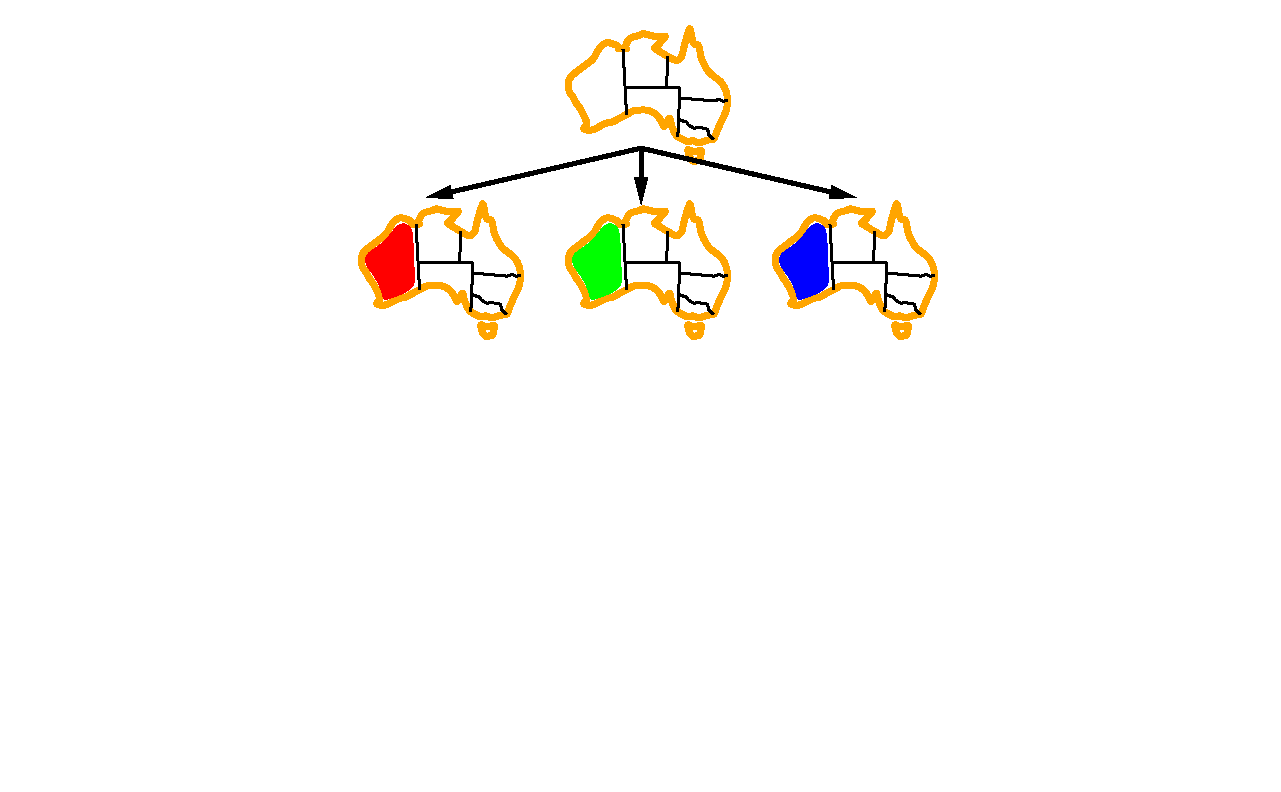
\includegraphics[width=4in]{backtrack-progress-2}}%
		\only<3>{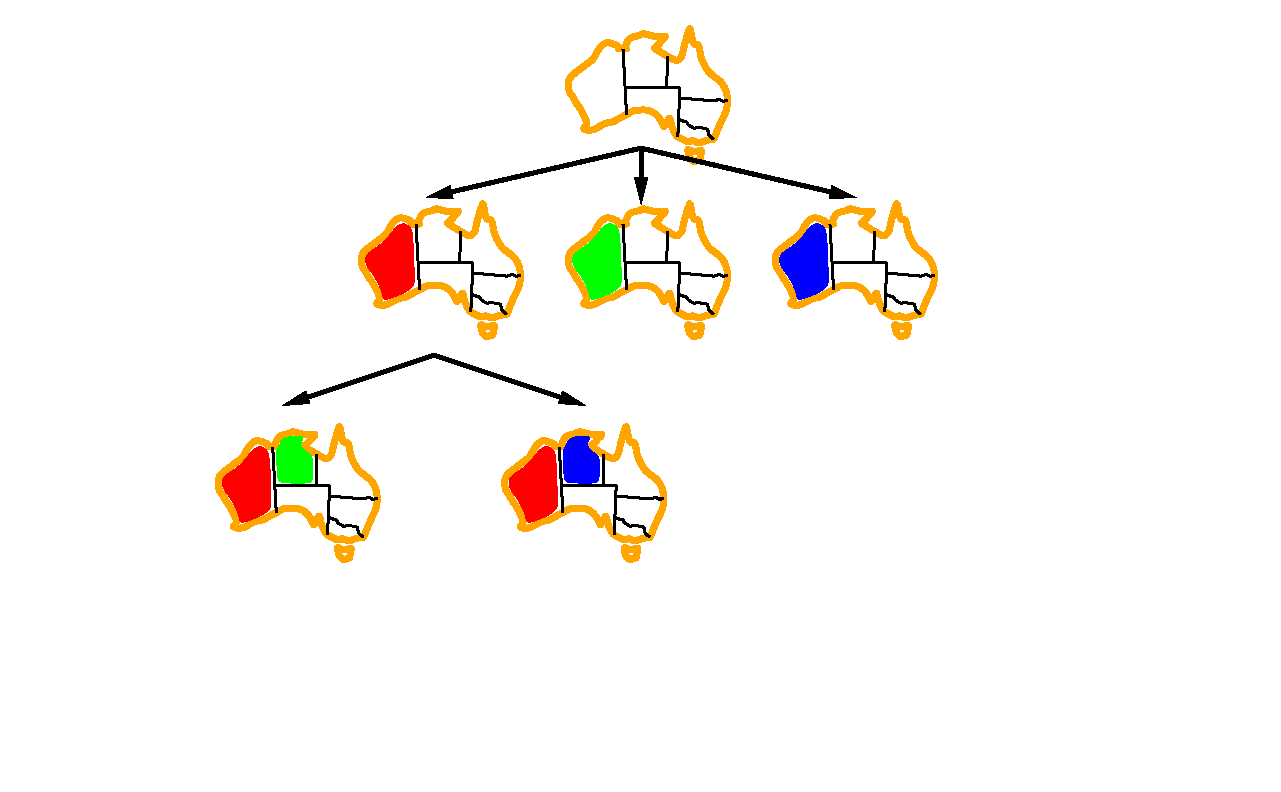
\includegraphics[width=4in]{backtrack-progress-3}}%
		\only<4>{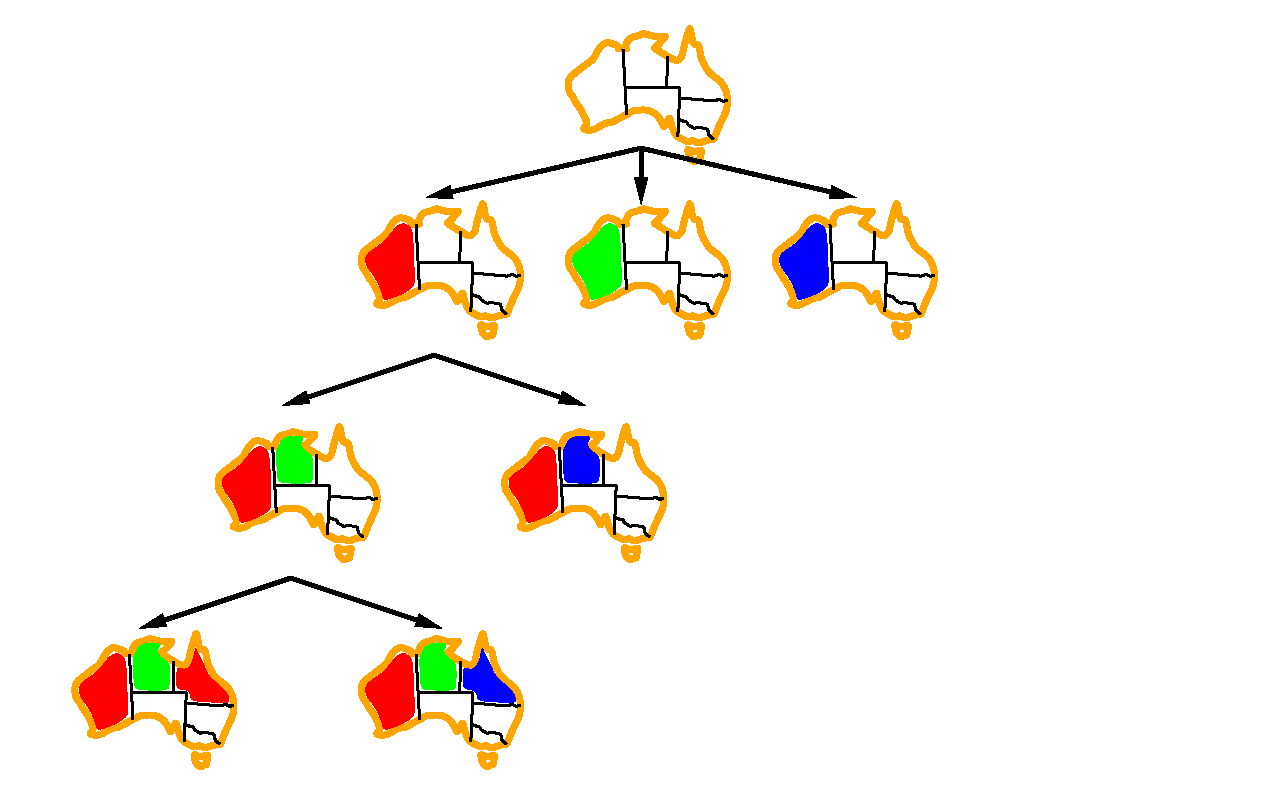
\includegraphics[width=4in]{backtrack-progress-4}}%
	\end{center}
\end{frame}

\subsection{Simple Search Heuristics}
\begin{frame}{Backtracking Heuristics}
	\begin{block}{Problem}
		\begin{itemize}
			\item Basic depth first search is still too inefficient.
			\item E.g. Can only solve $n$-queens for $n \approx 25$
		\end{itemize}
	\end{block}
	\begin{block}{How can we be smarter?}
		\begin{itemize}
			\pause
			\item Which variable should be assigned next?
			\pause
			\item In what order should its values be tried?
			\pause
			\item Can we detect inevitable failure early?
			\pause
			\item Can we take advantage of problem structure?
		\end{itemize}
	\end{block}
\end{frame}
\begin{frame}{Minimum Remaining Values}
	\begin{block}{Idea}
		Select the variable with the fewest legal values \\
	\end{block}
	\pause
	\begin{center}
		\visible<2->{
\includegraphics[width=4in]{australia-most-constrained-variable.pdf}}
	\end{center}
	\pause
	\begin{block}{Also Known As}
		Most Constrained Variable
	\end{block}
\end{frame}
\begin{frame}{Degree Heuristic}
	\begin{block}{Idea}
		\begin{itemize}
			\item But what to do when MRV produces ties?
			\item Select variable with most constraints on other values
		\end{itemize}
	\end{block}
	\pause
	\begin{center}
		\visible<2->{
\includegraphics[width=4in]{australia-most-constraining-variable.pdf}}
	\end{center}
	\pause
	\begin{block}{Also Known As}
		Most Constraining Variable
	\end{block}
\end{frame}
\begin{frame}{Least Constraining Value}
	\begin{block}{Idea}
		Select the variable that rules out the smallest
		number of values for the remaining variables
	\end{block}
	\pause
	\begin{center}
		\visible<2->{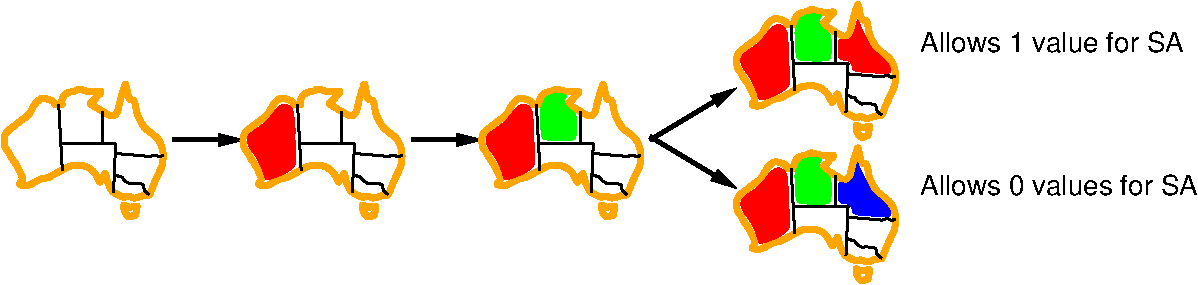
\includegraphics[width=4in]{australia-least-constraining-value.pdf}}
	\end{center}
	\pause
	\begin{tabular}{ll}
		          & Minimum Remaining Values \\
		+         & Degree Heuristic \\
		+         & Least Constraining Value \\
		\hline
		$\approx$ & 1000 queens
	\end{tabular}
\end{frame}

\subsection{Constraint Propogation}
\begin{frame}[t]{Forward Checking}
	\begin{block}{Idea}
		\begin{itemize}
			\item Keep track of remaining legal values for all variables
			\item Stop search when any variable has no legal values
		\end{itemize}
	\end{block}
	\only<1>{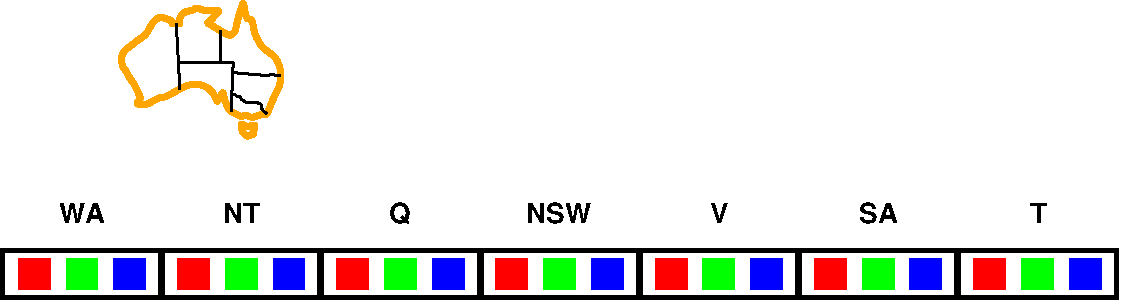
\includegraphics[width=4in]{forward-checking-progress-1.pdf}}%
	\only<2>{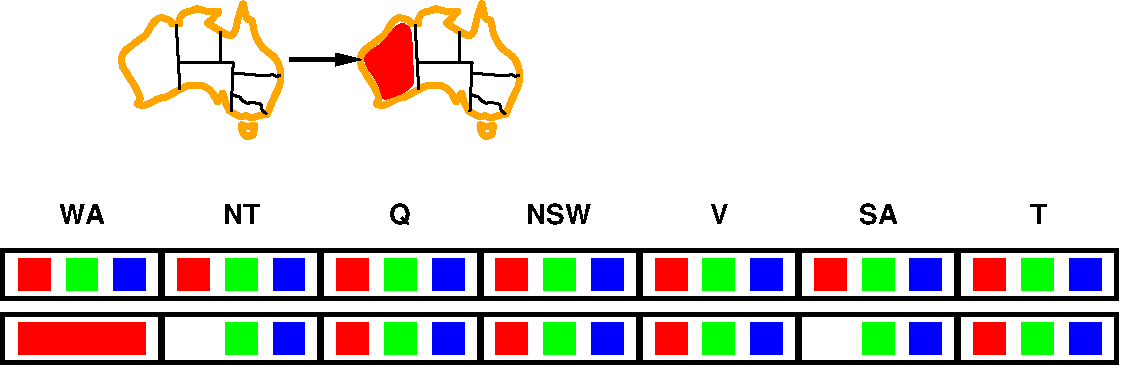
\includegraphics[width=4in]{forward-checking-progress-2.pdf}}%
	\only<3>{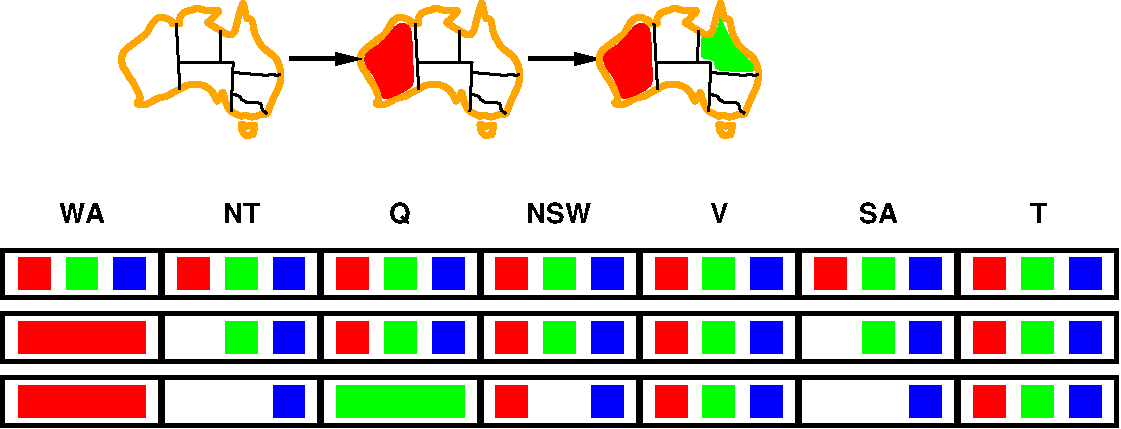
\includegraphics[width=4in]{forward-checking-progress-3.pdf}}%
	\only<4>{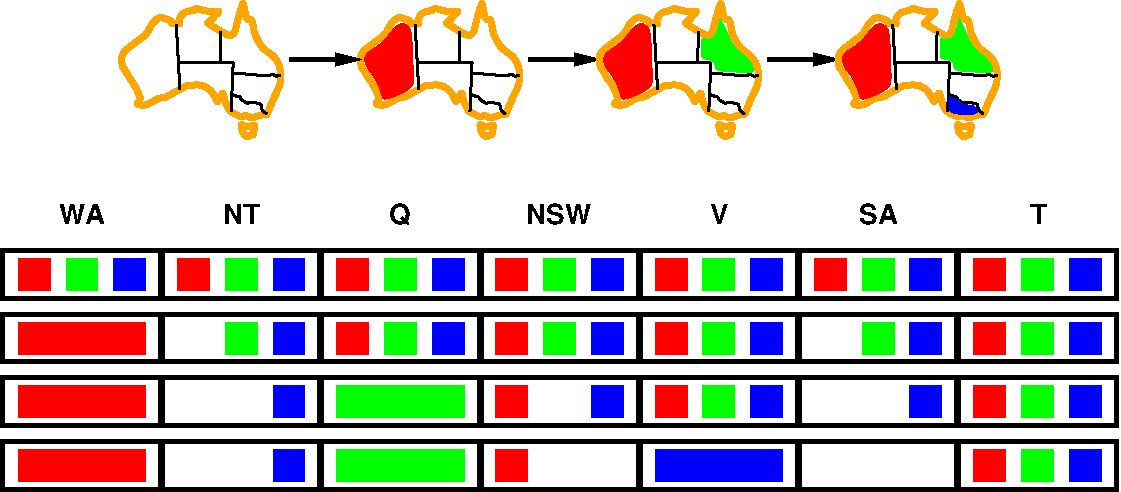
\includegraphics[width=4in]{forward-checking-progress-4.pdf}}%
\end{frame}
\begin{frame}{Constraint Propogation}
	\begin{block}{Problem with Forward Checking}
		\begin{itemize}
			\item Only propogates information from assigned variables
			\item<4-|alert@4-> Need to check constraints on unassigned variables!
		\end{itemize}
	\end{block}
	\begin{center}
		\visible<2->{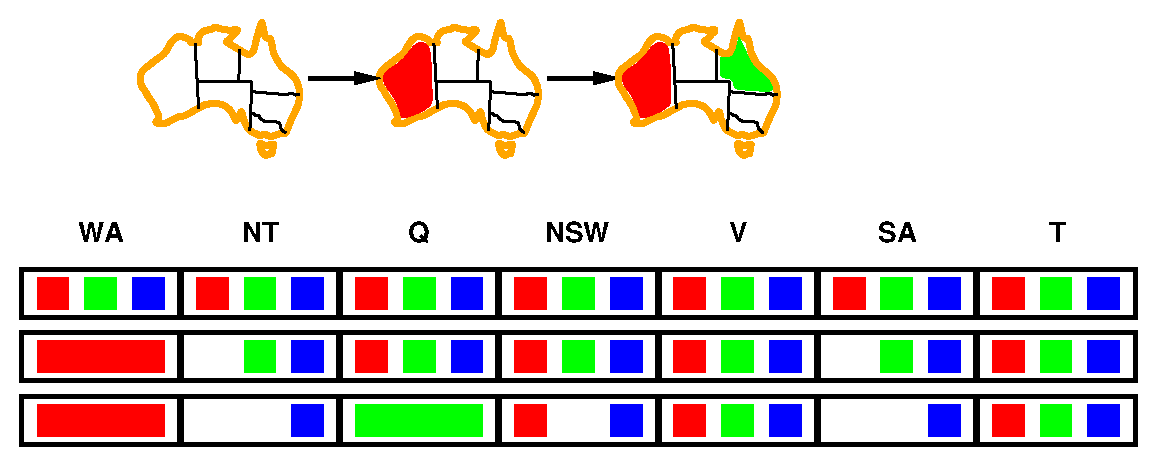
\includegraphics[width=4in]{forward-checking-progress-3}} \\
		\visible<3->{But \V{NT} and \V{SA} cannot both be blue!}
	\end{center}
\end{frame}
\begin{frame}{Arc Consistency}
	\begin{block}{$X \rightarrow Y$ is consistent iff}
		For \alert{every} value of $X$ there is \alert{some} legal value for $Y$
	\end{block}
	\begin{block}{Keeping Arcs Consistent}
		\begin{itemize}
			\item Remove domain values that make an arc inconsistent
			\item Check neighbors of variables with modified domains
		\end{itemize}
	\end{block}
	\only<1>{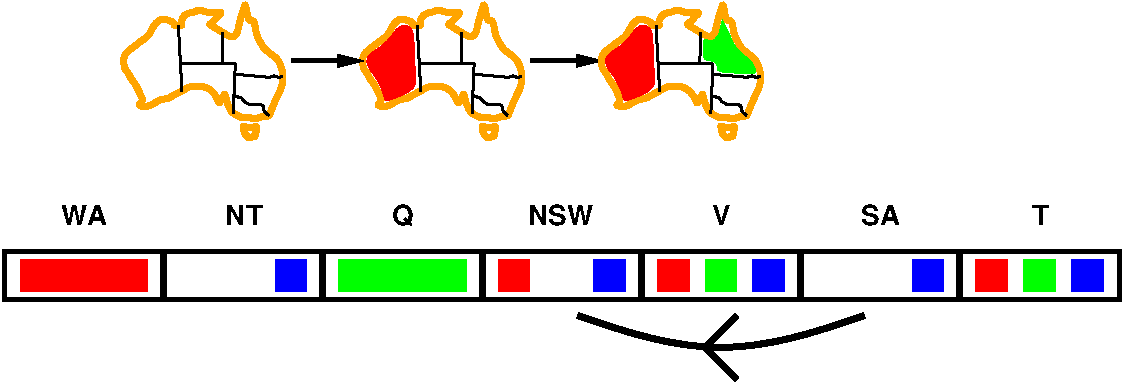
\includegraphics[width=4in]{arc-consistency-1.pdf}}%
	\only<2>{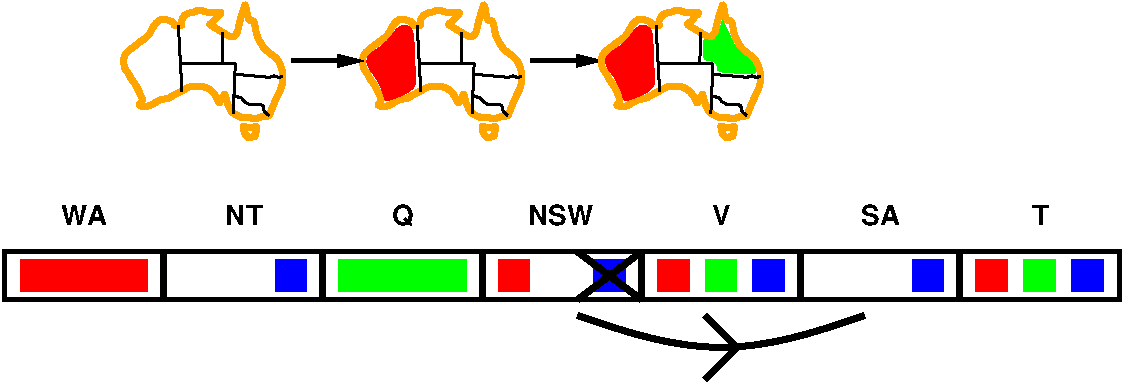
\includegraphics[width=4in]{arc-consistency-2.pdf}}%
	\only<3>{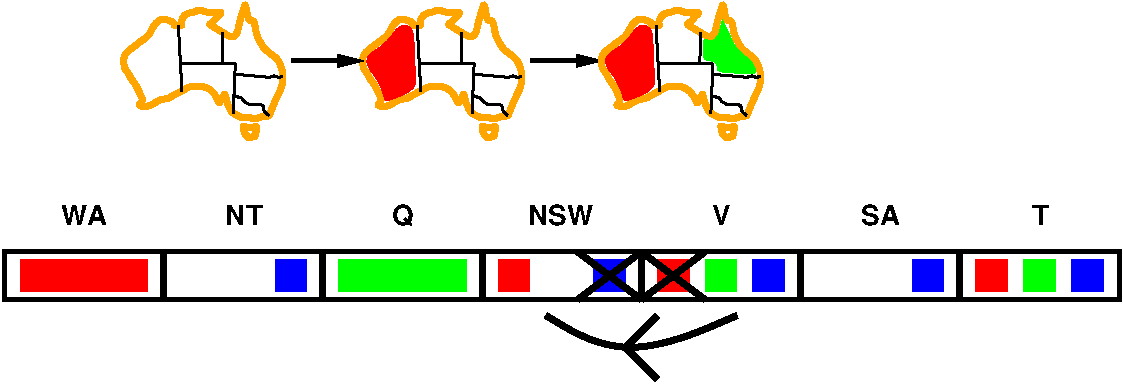
\includegraphics[width=4in]{arc-consistency-3.pdf}}%
	\only<4>{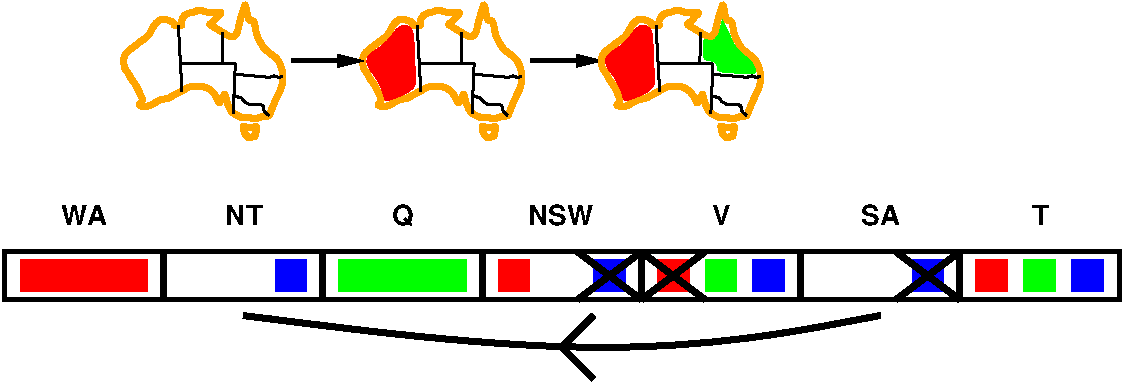
\includegraphics[width=4in]{arc-consistency-4.pdf}}%
\end{frame}
\begin{frame}[fragile]{Arc Consistency Code}
	\scriptsize
	\begin{semiverbatim}\bfseries
		\key{def} \defn{arc_consistency}(csp):
		    \pause\cmnt{# check all arcs in the CSP}
		    queue = collections.deque(csp.get_arcs())
		    \key{while} queue:
		        var1, var2 = queue.popleft()
		        \pause\cmnt{# if inconsistent values are found, add all neighbors}
		        \key{if} remove_inconsistent_values(csp, var1, var2):
		            \key{for} var3 \key{in} csp.get_neighbors(var1) - set([var2]):
		                queue.append(var3, var1)
		\pause
		\key{def} remove_inconsistent_values(csp, var1, var2):
		    \pause\cmnt{# search all the values of var1's domain}
		    removed = \key{False}
		    \key{for} value1 \key{in} var1.domain:
		        \pause\cmnt{# remove the value if it is inconsistent with var2}
		        \key{if} all(\key{not} csp.is_consistent(\{var1:value1, var2:value2\})
		               \key{for} value2 \key{in} var2.domain):
		            var1.domain.remove(value1)
		            removed = \key{True}
		    \pause\cmnt{# return whether or not any inconsistent values were removed}
		    \key{return} removed
	\end{semiverbatim}
\end{frame}
\begin{frame}{Properties of Arc Consistency Checking}
	Detects failure earlier than forward checking, but\ldots
	\begin{block}{Given $n$ variables, at most $d$ values per domain}
		\begin{itemize}
			\pause
			\item Maximum arcs in a binary CSP: \\
			      \pause \hspace{2em} $n^2$, all pairs
			\pause
			\item Maximum times an arc could be added to the queue: \\
			      \pause \hspace{2em} $d$, if all values in domain are deleted
			\pause
			\item Checking consistency of a single arc: \\
			      \pause \hspace{2em} $d^2$, all in $X_1$'s domain with all in $X_2$'s
			\pause
			\item Total time: \\
			      \pause \hspace{2em} $O(n^2d^3)$
		\end{itemize}
	\end{block}
\end{frame}
\begin{frame}{Arc Consistency Incompleteness}
	\begin{columns}
		\begin{column}{2in}
			\begin{block}{Problem}
				Arc consistency checking cannot detect some bad assignments, e.g. \\
				$\{\V{WA}=\V{red}, \V{NSW}=\V{red}\}$
			\end{block}
		\end{column}
		\begin{column}{2in}
			
\includegraphics[height=1.25in]{australia-arc-fail.pdf}
		\end{column}
	\end{columns}
	\pause
	\begin{block}{Partial Solution: Special Purpose Constraint Handling}
		\begin{itemize}
			\item Constraint: $\V{all-different}(\V{SA},\V{NT},\V{Q})$
			\item After arc consistency: $\V{SA}=\V{NT}=\V{Q}=\{\V{blue},\V{green}\}$
			\item Failure: \uncover<3>{\alert<3>{fewer values than variables!}}
		\end{itemize}
	\end{block}
\end{frame}

\section{Search Alternatives}

\subsection{Local Search}
\begin{frame}{CSPs as Local Search}
	\begin{block}{Formulation}
		\begin{description}
			\item[States] Complete assignments
			\item[Initial] Any complete assignment
			\item[Actions] Change value of one variable
			\item[Goal] Consistent assignment
		\end{description}
	\end{block}
	\pause
	\begin{block}{Benefits}
		\begin{itemize}
			\item Minimal memory consumption
			\item Emprically very effective
		\end{itemize}
	\end{block}
\end{frame}
\begin{frame}{Min-Conflicts}
	\begin{block}{Idea}
		\begin{itemize}
			\item Pick a variable with constraint violations
			\item Assign the value that violates the fewest constraints
		\end{itemize}
	\end{block}
	\begin{center}
		\visible<2>{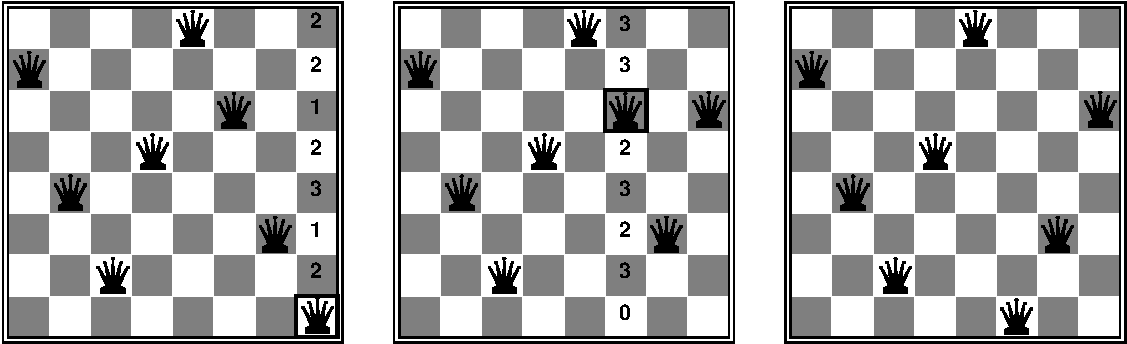
\includegraphics[width=4in]{8-queens-min-conflicts.pdf}}
	\end{center}
\end{frame}
\begin{frame}[fragile]{Min-Conflicts Code}
	\scriptsize
	\begin{semiverbatim}\bfseries
		\key{def} \defn{min_conflicts}(csp, max_steps):
		    \pause\cmnt{# start with an initial complete assignment}
		    assignment = \{\}
		    \key{for} variable \key{in} csp.variables:
		        assignment[variable] = random.choice(variable.domain)
		    \pause\cmnt{# adjust one variable each time through the loop}
		    \key{for} i \key{in} range(max_steps):
		        \pause\cmnt{# return the assignment when it is consistent}
		        \key{if} csp.is_consistent(assignment):
		            \key{return} assignment
		        \pause\cmnt{# otherwise, select a random conflicted variable}
		        var = random.choice(csp.get_conflicts(assignment))
		        \pause\cmnt{# assign the variable the value with minimal conflicts}
		        counts = \{\}
		        \key{for} value \key{in} var.domain:
		            assignment[var] = value
		            conflicts = csp.get_conflicts(assignment)
		            counts[value] = len(conflicts)
		        assignment[var] = min(counts, key=counts.get)
		    \pause\cmnt{# all assignments failed}
		    \key{return} \key{None}
	\end{semiverbatim}
\end{frame}
\begin{frame}{Min-Conflicts Properties}
	\begin{block}{$n$-Queens}
		Almost constant time for arbitrary $n$ with high probability
	\end{block}
	\pause
	\begin{block}{Other kinds of CSPs}
		\begin{columns}
			\begin{column}{1.5in}
				Appears the same is true except for a narrow range of:
				\[
					R = \frac{\left|\mbox{constraints}\right|}{\left|\mbox{variables}\right|}
				\]
			\end{column}
			\begin{column}{2in}
				\begin{center}
					\visible<2>{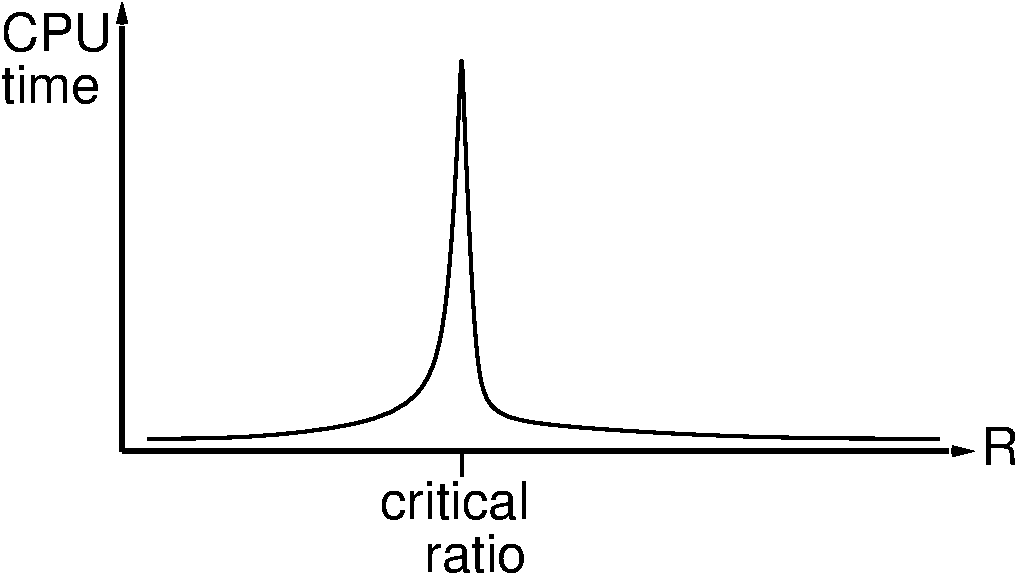
\includegraphics[width=2in]{random-csp-runtime.pdf}}
				\end{center}
			\end{column}
		\end{columns}
	\end{block}
\end{frame}

\subsection{Tree Search}
\begin{frame}{Tree-Structured CSPs}
	\begin{block}{Tree-Structured CSPs can be solved in polynomial time}
		\begin{enumerate}
			\item Choose one variable as the root
			\item List variables with parents before children, e.g.
				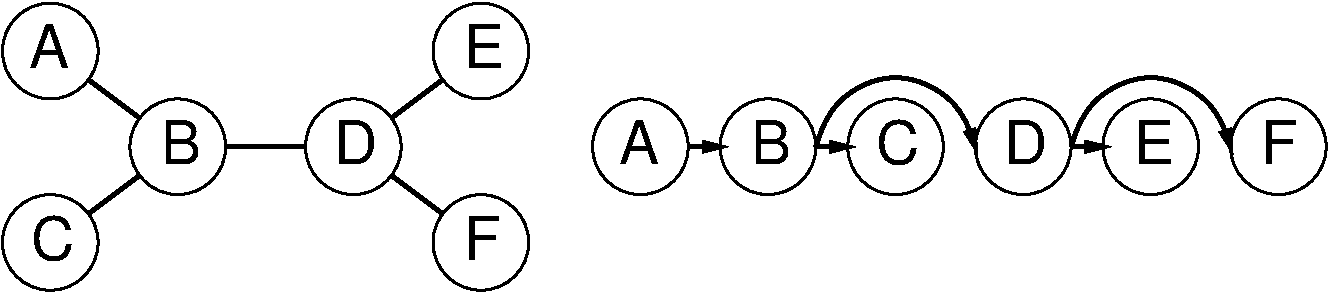
\includegraphics[width=3.5in]{tree-csp-2.pdf}
			\item Starting from the end, remove domain values inconsistent between parent and child
			\item Starting from the beginning, assign a value to each variable that is consistent with its parent
		\end{enumerate}
	\end{block}
\end{frame}
\begin{frame}{Tree-Structured CSP Example}
	\begin{block}{Schedule jobs A, B, C, D, E for 9, 10, 11 or 12}
		\begin{itemize}
			\item B must be before 11:00
			\item D must be after 10:00
			\item B \& C must be after A
			\item D \& E must be after C
		\end{itemize}
	\end{block}
	\begin{block}{Algorithm (Again)}
		\begin{enumerate}
			\item Choose one variable as the root
			\item List variables with parents before children
			\item From the end, remove inconsistent parent values
			\item From the start, assign values consistent with parents
		\end{enumerate}
	\end{block}
\end{frame}
\begin{frame}{Tree-Structured CSP Example}
	\begin{block}{Schedule jobs A, B, C, D, E for 9, 10, 11 or 12}
		\begin{itemize}
			\item B must be before 11:00
			\item D must be after 10:00
			\item B \& C must be after A
			\item D \& E must be after C
		\end{itemize}
	\end{block}
	\begin{center}
		\only<1>{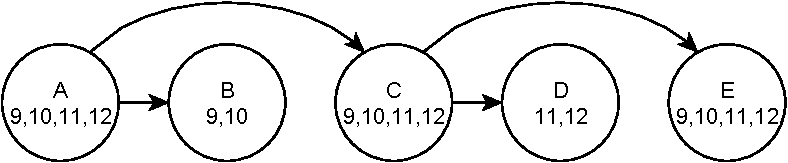
\includegraphics[width=4in]{tree-csp-solution-1.pdf}}%
		\only<2>{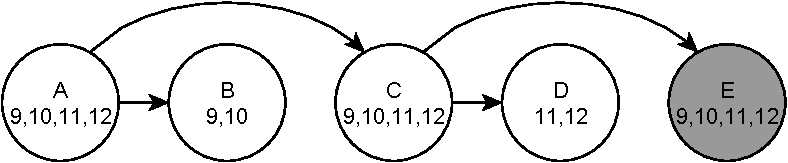
\includegraphics[width=4in]{tree-csp-solution-2.pdf}}%
		\only<3>{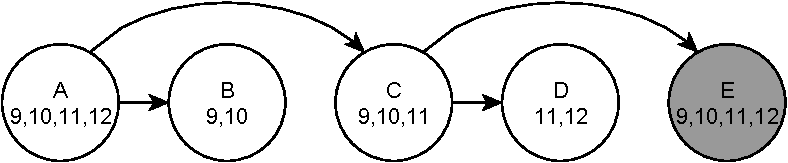
\includegraphics[width=4in]{tree-csp-solution-3.pdf}}%
		\only<4>{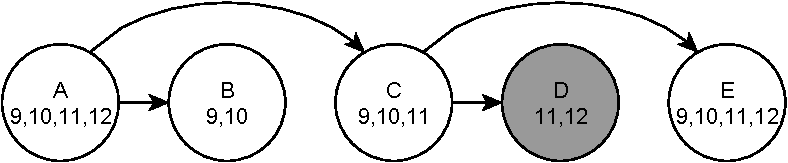
\includegraphics[width=4in]{tree-csp-solution-4.pdf}}%
		\only<5>{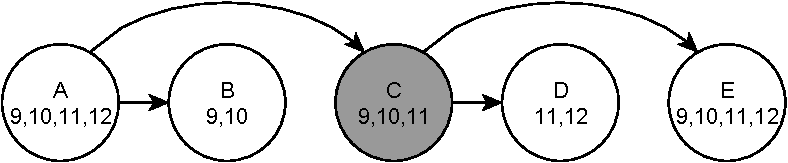
\includegraphics[width=4in]{tree-csp-solution-5.pdf}}%
		\only<6>{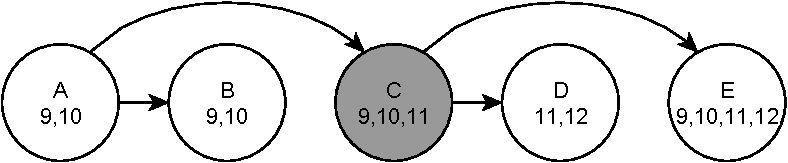
\includegraphics[width=4in]{tree-csp-solution-6.pdf}}%
		\only<7>{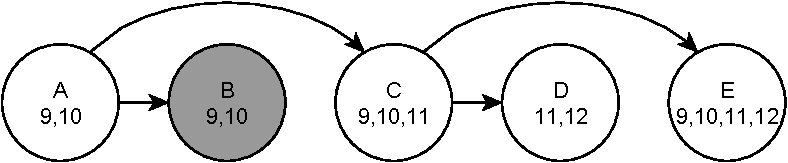
\includegraphics[width=4in]{tree-csp-solution-7.pdf}}%
		\only<8>{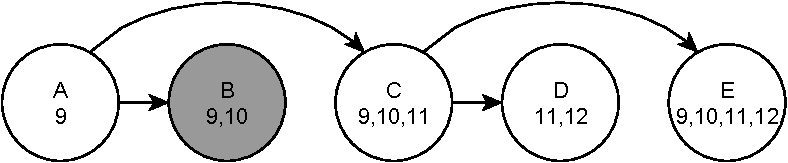
\includegraphics[width=4in]{tree-csp-solution-8.pdf}}%
		\only<9>{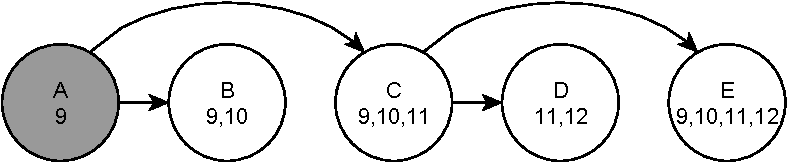
\includegraphics[width=4in]{tree-csp-solution-9.pdf}}%
		\only<10>{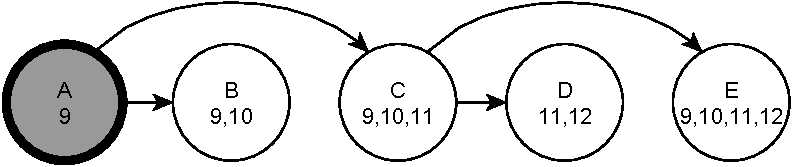
\includegraphics[width=4in]{tree-csp-solution-10.pdf}}%
		\only<11>{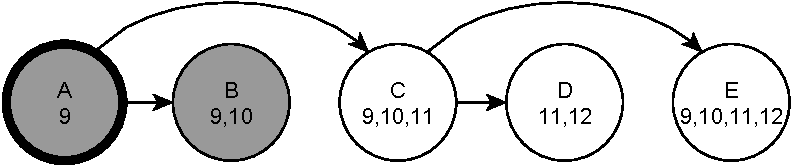
\includegraphics[width=4in]{tree-csp-solution-11.pdf}}%
		\only<12>{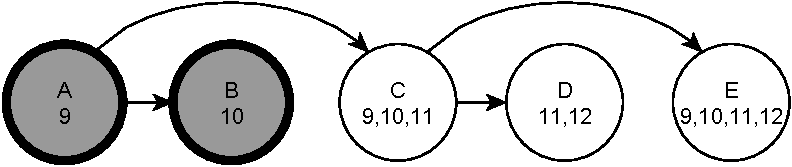
\includegraphics[width=4in]{tree-csp-solution-12.pdf}}%
		\only<13>{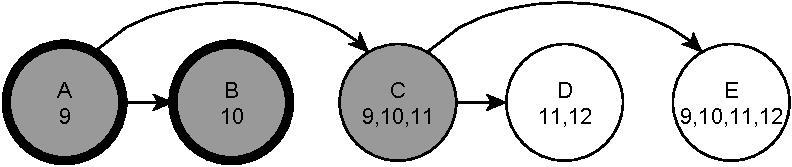
\includegraphics[width=4in]{tree-csp-solution-13.pdf}}%
		\only<14>{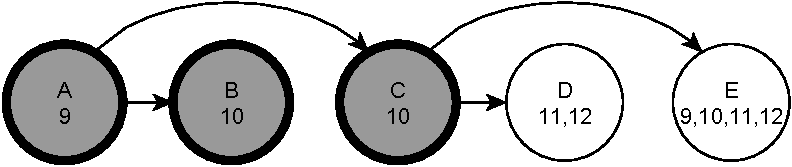
\includegraphics[width=4in]{tree-csp-solution-14.pdf}}%
		\only<15>{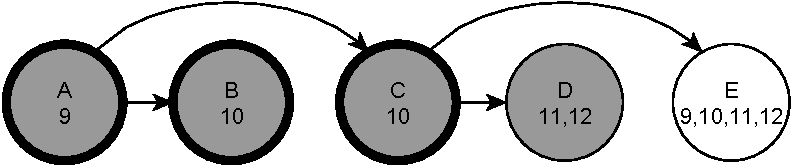
\includegraphics[width=4in]{tree-csp-solution-15.pdf}}%
		\only<16>{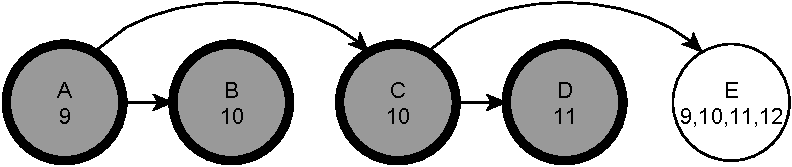
\includegraphics[width=4in]{tree-csp-solution-16.pdf}}%
		\only<17>{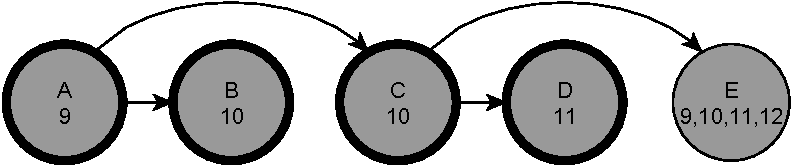
\includegraphics[width=4in]{tree-csp-solution-17.pdf}}%
		\only<18>{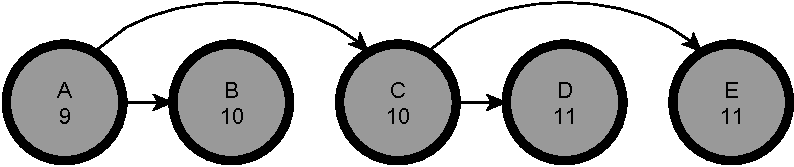
\includegraphics[width=4in]{tree-csp-solution-18.pdf}}%
	\end{center}
\end{frame}
\begin{frame}{Subproblems and Decomposition}
	\begin{columns}
		\begin{column}{2in}
			\begin{block}{Example}
				Tasmania and mainland are separate components
			\end{block}
			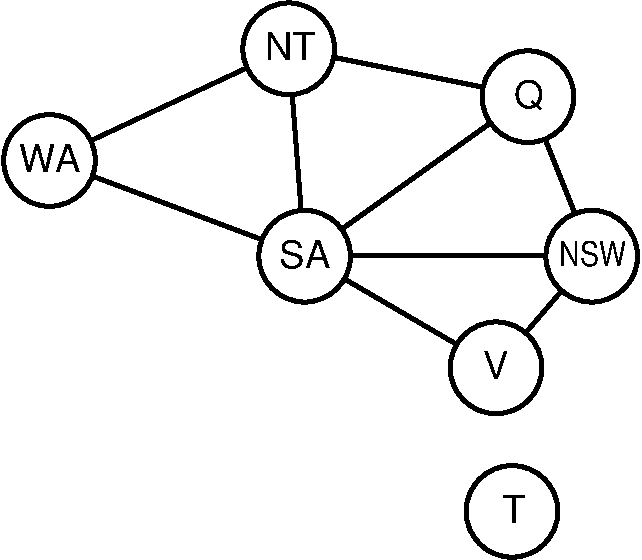
\includegraphics[width=2in]{australia-csp.pdf}
		\end{column}
		\begin{column}{2in}
			\begin{block}{If each subproblem has $c$ of the $n$ total variables}
				\begin{itemize}
					\pause\item Num. of subproblems:\\
					\pause\hspace{2em}$n/c$
					\pause\item Time per subproblem:\\
					\pause\hspace{2em}$d^c$
					\pause\item Total work: \pause$O(nd^c/c)$
				\end{itemize}
			\end{block}
			\pause
			\begin{block}{$n=80, d=2, c=20$}
				At 10 million nodes/sec:
				\begin{itemize}
					\item $2^{80} =$ 4 billion years 
					\item $4 \cdot 2^{20} =$ 0.4 seconds
				\end{itemize}
			\end{block}
		\end{column}
	\end{columns}
\end{frame}
\begin{frame}{Tree Decomposition}
	Convert constraint graphs to trees by assigning variables:
	\begin{center}
		\visible<2->{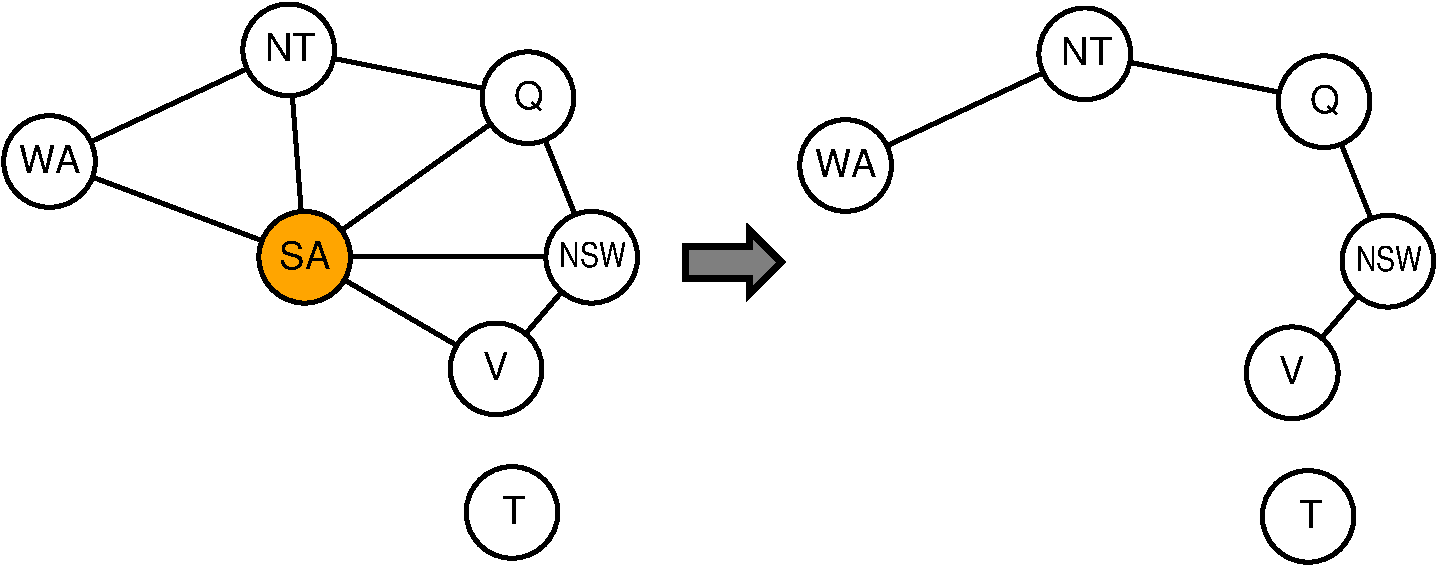
\includegraphics[width=3.5in]{australia-cutset.pdf}}
	\end{center}
	\begin{block}<3>{Properties}
		\begin{itemize}
			\item Complexity: \pause $O(d^c \cdot (n-c)d^2)$, given cutset size $c$
			\item Finding the smallest cycle cutset is NP-hard, but some efficient approximations exist
		\end{itemize}
	\end{block}
\end{frame}

\part{Key Points}
\begin{frame}{Key Points}
	\begin{block}{Constraint Satisfaction Problems}
		\begin{itemize}
			\item States are assignment of values to variables
			\item Goals are assignments with no constraint violations
		\end{itemize}
	\end{block}
	\begin{itemize}
		\item Backtracking \\			
			\begin{itemize}
				\item Depth-first search, one variable assigned per node
				\item Can be made effective with a number of heuristics
			\end{itemize}
		\item Min-Conflicts \\
			\begin{itemize}
				\item One value changed to reduce violations per iteration
				\item Usually effective in practice
			\end{itemize}
		\item Tree-Structured Search \\
			\begin{itemize}
				\item Can be solved in linear time
				\item Graphs can sometimes be decomposed into trees
			\end{itemize}
	\end{itemize}
\end{frame}

\end{document}


